\subsection{Neural Nets}

% Derivation from biology {{{
\subsubsection{Derivation from biology}
\label{ss_nn_derivation_from_biology}

"Neural networks are an attempt to model the insights
gained in brain research on the interaction between nerve
cells (neurons) and connections (synapses)".\cite{ct_math}

Here, an artificial neuron mimics the functioning of a
nerve cell . A biological nerve cell is connected to other
nerve cells via synapses. At these connections, stimuli are
transmitted by means of chemical messengers
(neurotransmitters) and converted into an electrical signal
within the nerve cell.

The synapses of a nerve cell are located at so-called
dendrites (branches), from which the transmitted stimuli
are transmitted to the soma (cell body). It does matter how
far the synapse is from the soma. The closer a synapse is
to the soma, the stronger the stimulus transmission.\cite{%
bio,ct_math}

In addition, it should be the case that multiple synapses
stimuli at the same time which adds incoming stimuli within
the nerve cell.\cite{bio} If the stimulus transmitted
exceeds a threshold within the cell, then an action
potential is triggered and the cell forwards the signal to
other cells, which in turn are connected via synapses to
the stimulating transmitting cell. Nerve cells form
associations in the human brain, which develop the ability
to recognize complex structures. Artificial neural networks
are an attempt to imitate these associations of nerve
cells.\cite{ct_math}
% }}}

% Structure of an artificial neuron {{{
\subsubsection{Structure of an artificial neuron}

\begin{figure}[H]
	\begin{center}
	\begin{tikzpicture}[%
    dot/.style={circle,draw,thick,fill=green!20}
  ]
		\node at (5,0) (out) {};
		\node at (0,0) [dot] (neuron) {$t=\sum_{i=1}^{n}{w_ix_i}$}
			edge[->,thick] node[above]{$\varphi(t-\theta)$} (out);
		\node at (-4,4) [dot] {$x_1$}
			edge[->,thick] (neuron);
		\node at (-4,2) [dot] {$x_2$}
			edge[->,thick] (neuron);
		\node at (-4,0) [dot] {$x_3$}
			edge[->,thick] (neuron);
		\node at (-4,-4) [dot] {$x_n$}
			edge[->,thick] (neuron);
		\node at (-4,-1.5) [tokens=1] {};
		\node at (-4,-2) [tokens=1] {};
		\node at (-4,-2.5) [tokens=1] {};
	\end{tikzpicture}
	\end{center}
	\caption{Scheme of an artificial neuron}
	\label{fig_neuron}
\end{figure}



From chapter \ref{ss_nn_derivation_from_biology}, the
components and functioning of an artificial neuron can be
derived.
\newline\newline
In an artificial neuron the following happens:

\begin{enumerate}

  \item An artificial neuron is connected to other neurons
        or the direct value input via input connections,
        which are supposed to represent the synapses of the
        nerve cell (described in Figure \ref{fig_neuron}
        with $x_i$). These inputs can be discreet or
        continuous.\cite{nne_beck}

        If the data comes from other neurons, the weighting
        of the connection is additionally transferred to
        the value $\omega_i$ . Each connection of a neuron
        has an individual weighting. The greater the value
        of this weighting, the more important the
        transmitted value $x_i$ for the network output.

  \item The value and weight of each input connection is
        added by the transfer function $\sum_{i=1}^{n}w_ix_i$
        to calculate the net input value $t$.


  \item Every artificial neuron, like a nerve cell, has a
        threshold. An artificial neuron is a value
        $\theta$. The threshold $\theta$ is subtracted from
        the net input value $t$ to determine the activation
        potential of the neuron.

        The threshold can also be represented by the bias.
        The bias is a further input, which transmits the
        constant value 1 and as weighting the value
        $b=-\theta$.

        	\begin{figure}[H]
		\begin{center}
			\begin{tikzpicture}[dot/.style={circle,draw,thick,fill=green!20,minimum size=1cm}]
				\node at (5,0) (out) {};
				\node at (0,0) [dot] (neuron) {$t=\sum_{i=1}^{n}{w_ix_i}+b$}
					edge[->,thick] node[above]{$\varphi(t)$} (out);
				\node at (-4,4) [dot] {$1$}
					edge[->,thick] node[anchor=south west]{$b=-\theta$} (neuron);
				\node at (-4,2) [dot] {$x_1$}
					edge[->,thick] (neuron);
				\node at (-4,0) [dot] {$x_2$}
					edge[->,thick] (neuron);
				\node at (-4,-4) [dot] {$x_n$}
					edge[->,thick] (neuron);
				\node at (-4,-1.5) [tokens=1] {};
				\node at (-4,-2) [tokens=1] {};
				\node at (-4,-2.5) [tokens=1] {};
			\end{tikzpicture}
		\end{center}
    \caption{An artificial neuron with bias}
    %\label{bn}
	\end{figure}



  \item The determined value of $t-\theta$ is used as an
        input in the activation function to determine the
        output of the neuron.

        From this process, the basic elements of a neuron
        can be determined:

        \begin{itemize}

          \item Weighting

          \item Threshold

          \item Transfer function

          \item Activation function

        \end{itemize}

\end{enumerate}
% }}}

% Construction of a neural network {{{
\subsubsection{Construction of a neural network}

\begin{figure}[H]
  \begin{center}
	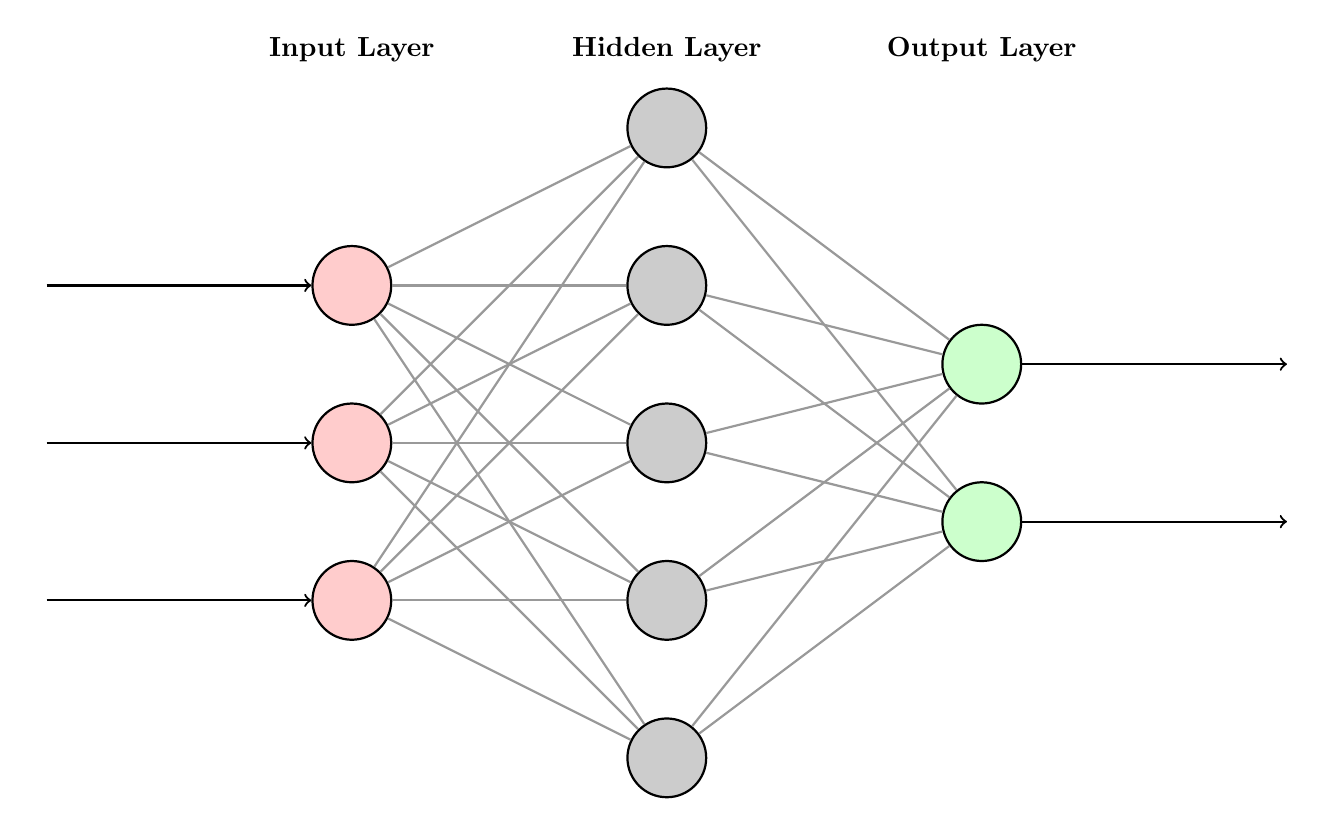
\begin{tikzpicture}[%
    dot/.style={circle,draw,thick,minimum size = 1cm}
  ]
		\node at(-4,5) {\textbf{Input Layer}};
		\node at(0,5) {\textbf{Hidden Layer}};
		\node at(4,5) {\textbf{Output Layer}};

		\node at(8,1) (oo1) {};
		\node at(8,-1) (oo2) {};

		\node at (4,1) [dot,fill=green!20] (o1) {}
			edge[->,thick] (oo1);
		\node at (4,-1) [dot,fill=green!20] (o2) {}
			edge[->,thick] (oo2);

		\node at (0,4) [dot,fill=black!20] (h1) {}
			edge[thick,black!40] (o1)
			edge[thick,black!40] (o2);
		\node at (0,2) [dot,fill=black!20] (h2) {}
			edge[thick,black!40] (o1)
			edge[thick,black!40] (o2);
		\node at (0,0) [dot,fill=black!20] (h3) {}
			edge[thick,black!40] (o1)
			edge[thick,black!40] (o2);
		\node at (0,-2) [dot,fill=black!20] (h4) {}
			edge[thick,black!40] (o1)
			edge[thick,black!40] (o2);
		\node at (0,-4) [dot,fill=black!20] (h5) {}
			edge[thick,black!40] (o1)
			edge[thick,black!40] (o2);

		\node at (-4,2) [dot,fill=red!20] (i1) {}
			edge[thick,black!40] (h1)
			edge[thick,black!40] (h2)
			edge[thick,black!40] (h3)
			edge[thick,black!40] (h4)
			edge[thick,black!40] (h5);
		\node at (-4,0) [dot,fill=red!20] (i2) {}
			edge[thick,black!40] (h1)
			edge[thick,black!40] (h2)
			edge[thick,black!40] (h3)
			edge[thick,black!40] (h4)
			edge[thick,black!40] (h5);
		\node at (-4,-2) [dot,fill=red!20] (i3) {}
			edge[thick,black!40] (h1)
			edge[thick,black!40] (h2)
			edge[thick,black!40] (h3)
			edge[thick,black!40] (h4)
			edge[thick,black!40] (h5);

		\node at(-8,2) (ii1) {}
			edge[->,thick] (i1);
		\node at(-8,0) (ii2) {}
			edge[->,thick] (i2);
		\node at(-8,-2) (ii3) {}
			edge[->,thick] (i3);
	\end{tikzpicture}
  \end{center}
  \caption{Neural network with hidden layer}
  %\label{snn}
\end{figure}


Neural networks are built in several levels (layers). Each
of these layers consists of a certain number of neurons and
connections. Each neuron of a layer is connected to all
neurons of the next layer via the already discussed
weighted input connections.

\begin{itemize}

  \item \textbf{Input layer:}

        The input layer is the first layer of a neural
        network. It contains the same Number of neurons,
        such as input and output values in the test and
        learning data available.

  \item \textbf{Hidden layer:}

        A neural network can not contain, one or more
        hidden layers. Neural networks can solve simple
        problems without hidden layers, many problems, such
        as the so-called "XOR problem", can't be solved
        without at least one of these layers.\cite{nne_beck}

        The hidden layers consist of neurons, which
        together represent an internal representation of
        the input. The weighting to the individual neurons
        of the hidden layer is determined, for example, by
        means of back propagation.

  \item \textbf{Output-Layer:}

        The output layer is the last layer of a neural
        network. It delivers the results of the network to
        the outside world. The number of neurons in the
        output layer equals the number of expected output
        values.

\end{itemize}
% }}}

% Learning algorithms {{{
\subsubsection{Learning algorithms}

Each neural network must be trained with training records.
These records consist of rows with the input values and the
expected output (supervised learning). The training itself
is an iterative process in which each input and output
passes through rows.\cite{ct_math}

In order for the network to learn how to approximate the
output value, the weights and threshold of each neuron must
be modified and adjusted.

The quality measure is the quadratic cost function:

\begin{align*}
  E = \frac{1}{2}\sum_{i=1}^{n}(a_i-o_i)^2
\end{align*}

The network error $E$ consists of the accumulated squared
deviations of the individual rows.

These are calculated from the difference between the
expected output value $a_i$ and the calculated network
output $o_i$. The sum is multiplied by $\frac{1}{2}$. This
factor simplifies the derivation. The aim now is to find
the combination of thresholds and weights of the neurons in
which the network error $E$ is the lowest.

You could now let the net simply try all possible weights
and thresholds until the combination with the smallest
error $E$ is found. This is not possible in practice, as
there are usually too many parameters that have to be tried
out within the network.\cite{ct_math}

For this purpose, learning algorithms are used instead.
Learning algorithms distinguish between two categories,
supervised and unsupervised learning.
% }}}

% Reinforcement learning {{{
\subsubsection{Reinforcement Learning}

Reinforcement learning (RL) is an area of machine learning,
inspired by behaviorist psychology, concerned with how
software agents ought to take actions in an environment so
as to maximize some notion of cumulative reward.

The problem, due to its generality, is studied in many
other disciplines, such as game theory, control theory,
operations research, information theory, simulation-based
optimization, multi-agent systems, swarm intelligence,
statistics and genetic algorithms. In the operations
research and control literature, reinforcement learning is
called approximate dynamic programming, or neuro-dynamic
programming.

The problems of interest in reinforcement learning have
also been studied in the theory of optimal control, which
is concerned mostly with the existence and characterization
of optimal solutions, and algorithms for their exact
computation, and less with learning or approximation,
particularly in the absence of a mathematical model of the
environment. In economics and game theory, reinforcement
learning may be used to explain how equilibrium may arise
under bounded rationality.\cite{wrl}

While neural networks are responsible for recent
breakthroughs in problems like computer vision, machine
translation and time series prediction – they can also
combine with reinforcement learning algorithms to create
something astounding like AlphaGo.\cite{alphago}

Reinforcement learning refers to goal-oriented algorithms,
which learn how to attain a complex objective (goal) or
maximize along a particular dimension over many steps; for
example, maximize the points won in a game over many moves.
They can start from a blank slate, and under the right
conditions they achieve superhuman performance. Like a
child incentivized by spankings and candy, these algorithms
are penalized when they make the wrong decisions and
rewarded when they make the right ones – this is
reinforcement. Reinforcement algorithms that incorporate
deep learning can beat world champions at the game of Go as
well as human experts playing numerous Atari video games.
While that may sound trivial, it’s a vast improvement over
their previous accomplishments, and the state of the art is
progressing rapidly.\cite{alphago}

Reinforcement learning solves the difficult problem of
correlating immediate actions with the delayed returns they
produce. Like humans, reinforcement learning algorithms
sometimes have to wait a while to see the fruit of their
decisions. They operate in a delayed return environment,
where it can be difficult to understand which action leads
to which outcome over many time steps.

Reinforcement learning algorithms can be expected to
perform better and better in more ambiguous, real-life
environments while choosing from an arbitrary number of
possible actions, rather than from the limited options of a
video game. That is, with time we expect them to be
valuable to achieve goals in the real world.\cite{aiw}
% }}}

% Neural Networks and Deep Reinforcement Learning {{{
\subsubsection{Neural Networks and Deep Reinforcement
  Learning}
\label{ss_nn_nndrl}

Where do neural networks fit in with RL? Neural networks
are the agent that learns to map state-action pairs to
rewards. Like all neural networks, they use coefficients to
approximate the function relating inputs to outputs, and
their learning consists to finding the right coefficients,
or weights, by iteratively adjusting those weights along
gradients that promise less error.

In reinforcement learning, convolutional networks can be
used to recognize an agent's state; e.g.\ the screen that
Mario is on, or the terrain before a drone. That is, they
perform their typical task of image recognition.

But convolutional networks derive different interpretations
from images in reinforcement learning than in supervised
learning. In supervised learning, the network applies a
label to an image; that is, it matches names to pixels.

In reinforcement learning, given an image that represents a
state, a convolutional net can rank the actions possible to
perform in that state; for example, it might predict that
running right will return 5 points, jumping 7, and running
left none.

\begin{figure}[H]
  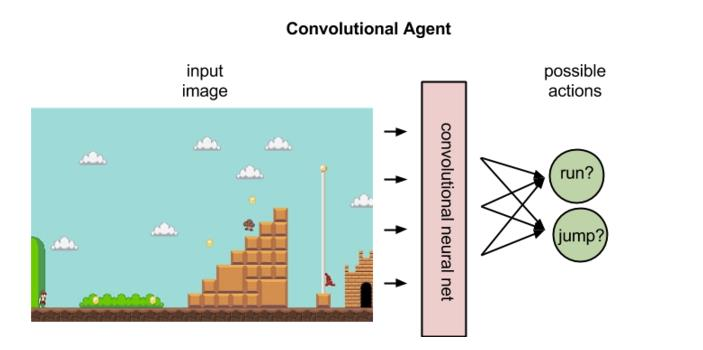
\includegraphics[width=\linewidth]{%
    diagrams/convolution_agent.PNG}
  \caption{Convolutional Agent\cite{aiw}}
\end{figure}

The above image illustrates what a policy agent does,
mapping a state to the best action.


At the beginning of reinforcement learning, the neural
network coefficients may be initialized stochastically, or
randomly. Using feedback from the environment, the neural
net can use the difference between its expected reward and
the ground-truth reward to adjust its weights and improve
its interpretation of state-action pairs.

Reinforcement learning relies on the environment to send it
a scalar number in response to each new action. The rewards
returned by the environment can be varied, delayed or
affected by unknown variables, introducing noise to the
feedback loop.\cite{aiw}

\begin{figure}[H]
  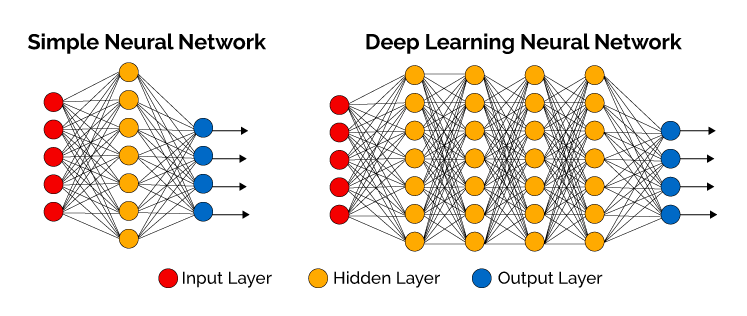
\includegraphics[width=\linewidth]{%
    diagrams/deep_learning.png}
  \caption{Difference between a Deep Learning Network and
    a Neural Network}
\end{figure}

The typical framing of a Reinforcement Learning (RL)
scenario: an agent takes actions in an environment, which
is interpreted into a reward and a representation of the
state, which are fed back into the agent.

\begin{figure}[H]
  \centering
  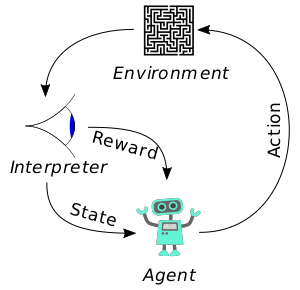
\includegraphics[width=\linewidth/2]{%
    diagrams/reinforcement_learning.png}
  \caption{Reinforcement learning diagram\cite{wrl}}
\end{figure}
% }}}
